%==============================================================================
%  Homework template  --  999 Controls
%
%  To reuse for the next assignment:
%    1. copy this folder,  2. edit the METADATA block below,
%    3. edit the SOLUTIONS section,  4. run  `make`.
%
%  Build:  make          (regenerates code output, then builds main.pdf)
%          make clean    (removes build artifacts)
%==============================================================================
\documentclass[11pt,letterpaper]{article}

%------------------------------- METADATA -------------------------------------
\newcommand{\hwcourse}{EE 999 --- Introduction to Control Systems}
\newcommand{\hwcourseshort}{EE 999}  % running head, keep it short
\newcommand{\hwtitle}{Homework 4}
\newcommand{\hwauthor}{Patrick Gordon}
\newcommand{\hwdate}{\today}
\newcommand{\hwdue}{Due Wednesday, October 7, 2026}
%------------------------------------------------------------------------------

\usepackage[T1]{fontenc}
\usepackage[utf8]{inputenc}
\usepackage{textcomp}
\usepackage[letterpaper,margin=1in,headheight=14pt]{geometry}
\usepackage{amsmath,amssymb}
\usepackage{cancel}
\usepackage{array}
\usepackage{graphicx}
\usepackage[american]{circuitikz}
\usepackage{xcolor}
\usepackage{listings}
\usepackage{fancyhdr}
\usepackage{inconsolata}
\usepackage{pdflscape}
\usepackage{float}
\usepackage[hidelinks]{hyperref}

%--- page furniture -----------------------------------------------------------
\pagestyle{fancy}
\fancyhf{}
\lhead{\hwauthor}
\chead{\hwtitle}
\rhead{\hwcourseshort}
\cfoot{\thepage}

%--- listing styles -----------------------------------------------------------
\definecolor{codebg}{HTML}{F7F7F4}
\definecolor{outbg}{HTML}{FCFCFC}
\definecolor{rule}{HTML}{C8C8C0}
\definecolor{kw}{HTML}{1C4FA1}
\definecolor{cmt}{HTML}{6A7A5A}
\definecolor{str}{HTML}{A0522D}

\lstdefinestyle{mcode}{
  language=Octave,
  basicstyle=\ttfamily\footnotesize,
  keywordstyle=\color{kw}\bfseries,
  commentstyle=\color{cmt}\itshape,
  stringstyle=\color{str},
  backgroundcolor=\color{codebg},
  frame=single,
  rulecolor=\color{rule},
  framesep=6pt,
  numbers=left,
  numberstyle=\ttfamily\scriptsize\color{gray},
  numbersep=8pt,
  showstringspaces=false,
  breaklines=true,
  columns=fullflexible,
  keepspaces=true,
  upquote=true,
}

\lstdefinestyle{moutput}{
  basicstyle=\ttfamily\footnotesize,
  backgroundcolor=\color{outbg},
  frame=single,
  rulecolor=\color{rule},
  framesep=6pt,
  showstringspaces=false,
  breaklines=true,
  columns=fullflexible,
  keepspaces=true,
  upquote=true,
}

%--- structure helpers --------------------------------------------------------
% \problem{1.1b}{Optional title}
\newcommand{\problem}[2]{%
  \bigskip
  \noindent{\large\bfseries Problem #1}%
  \ifx\relax#2\relax\else\ {\large --- #2}\fi
  \par\nobreak\vspace{2pt}\hrule\vspace{8pt}\nobreak
}

% \caplabel{Code}{hw_02_A.m}
\newcommand{\caplabel}[2]{%
  \par\nobreak\vspace{6pt}\nobreak
  \noindent{\small\bfseries #1}\ {\small\ttfamily \detokenize{#2}}%
  \par\nobreak\vspace{2pt}\nobreak
}

% \matlabcode{hw_02_A.m}  -- source listing pulled straight from the .m file
\newcommand{\matlabcode}[1]{%
  \caplabel{Code:}{#1}%
  \lstinputlisting[style=mcode]{#1}%
}

% \codeoutput{output/hw_02_A.txt} -- console output captured by the Makefile
\newcommand{\codeoutput}[1]{%
  \caplabel{Output:}{#1}%
  \IfFileExists{#1}{\lstinputlisting[style=moutput]{#1}}{\missing{#1}{run \texttt{make} to generate it}}%
}

% \answerfigure[width]{figures/foo.pdf}{Caption}  -- placeholder if not exported
% yet. Any format graphicx reads works: pdf, png, jpg.
% A script that plots is exported by the Makefile to figures/<script>.pdf, so
% \answerfigure{figures/hw_02_F.pdf}{...} is how a plotted answer is included.
% The optional argument is the printed width, default the full text width.
% Give a scan or screenshot a smaller one so it is not blown up past its own
% resolution:  \answerfigure[0.8\linewidth]{figures/some_scan.png}{...}
\newcommand{\answerfigure}[3][\linewidth]{%
  \begin{figure}[H]
    \centering
    \IfFileExists{#2}{\includegraphics[width=#1]{#2}}{\missing{#2}{export it, see README}}
    \caption{#3}
  \end{figure}%
}

%--- tables -------------------------------------------------------------------
% Centred paragraph column, so a description column wraps instead of running
% off the page:  \begin{tabular}{|c|P{0.5\linewidth}|}
\newcolumntype{P}[1]{>{\centering\arraybackslash}p{#1}}

% \begin{symboltable}{Signal}{Caption}  -- the symbol / units / description
% table used to define the variables of a problem. The first argument is the
% heading of the left column (Signal, Parameter, State, ...); leave the second
% empty for no caption.
%
%   \begin{symboltable}{Signal}{}
%     \sym{x(t)}{m}{Position of tire center}
%     \sym{r(t)}{m}{Road height (depends on $v_{car}(t)$)}
%   \end{symboltable}
%
% \sym puts its first argument in math mode and brackets the units, so write
% \sym{x(t)}{m}{...}, not \sym{$x(t)$}{[m]}{...}. Anything already math -- a
% subscript, a fraction -- goes in the description as usual: $\frac{1}{4}$.
%
% The optional argument is the width of the description column, for a table
% whose descriptions are much longer or much shorter than average:
%   \begin{symboltable}[0.35\linewidth]{Parameter}{}
\newcommand{\sym}[3]{$#1$ & [#2] & #3 \\ \hline}
\newenvironment{symboltable}[3][0.45\linewidth]{%
  \def\symtabcap{#3}%
  \begin{table}[H]
  \centering
  \renewcommand{\arraystretch}{1.4}
  \begin{tabular}{|c|c|P{#1}|}
  \hline
  #2 & Units & Description \\ \hline\hline
}{%
  \end{tabular}
  \ifx\symtabcap\empty\else\caption{\symtabcap}\fi
  \end{table}%
}

% \begin{answertable}{|c|c|c|}{Caption} -- any other table. Same placement and
% captioning as \answerfigure, but you write the rows yourself:
%
%   \begin{answertable}{|c|P{0.5\linewidth}|}{Pole locations.}
%     \hline
%     Pole & Behaviour \\ \hline\hline
%     $s=-2$ & decays in half a second \\ \hline
%   \end{answertable}
\newenvironment{answertable}[2]{%
  \def\anstabcap{#2}%
  \begin{table}[H]
  \centering
  \renewcommand{\arraystretch}{1.4}
  \begin{tabular}{#1}
}{%
  \end{tabular}
  \ifx\anstabcap\empty\else\caption{\anstabcap}\fi
  \end{table}%
}

% \begin{termtable}{4}{Caption} -- collect like powers of $s$ when multiplying
% out a characteristic polynomial (or any other expansion). The argument is the
% highest power; the columns and the $s^4 \dots s^0$ header are generated from
% it, so changing the degree is a one-character edit. Leave the second argument
% empty for no caption.
%
% Cells are already in math mode: write m_1m_2, not $m_1m_2$. One row per factor
% you multiplied out, one column per power; leave a cell empty where that factor
% contributes nothing to that power. Rows end with \\, like any tabular.
%
%   \begin{termtable}{4}{Terms of the characteristic polynomial.}
%     m_1m_2 & m_1b & m_1k_s       & bk_s       & k_s(k_s+k_w) \\
%            & m_2b & m_2(k_s+k_w) & b(k_s+k_w) &              \\
%            &      & -b^2         & -bk_s      & -k_s^2
%   \end{termtable}
%
% M is a centred column that is always in math mode. It uses \( \) rather than
% $ $ so that an empty cell stays empty -- a bare $$ would start display math.
\newcolumntype{M}{>{\(}c<{\)}}
\makeatletter
\newcount\tt@i
\newcommand{\tt@cols}{}
\newcommand{\tt@head}{}
\newcommand{\tt@build}[1]{%
  \def\tt@cols{}\def\tt@head{}%
  \tt@i=#1\relax
  \@whilenum\tt@i>\m@ne\do{%
    \edef\tt@cols{\tt@cols M}%
    \ifx\tt@head\@empty
      \edef\tt@head{s^{\the\tt@i}}%
    \else
      \edef\tt@head{\tt@head & s^{\the\tt@i}}%
    \fi
    \advance\tt@i\m@ne
  }%
}
\newenvironment{termtable}[2]{%
  \def\tt@cap{#2}%
  \tt@build{#1}%
  \begin{table}[H]%
  \centering
  \setlength{\tabcolsep}{12pt}%
  \renewcommand{\arraystretch}{1.3}%
  \edef\@tempa{\noexpand\begin{tabular}{\tt@cols}}\@tempa
  \tt@head \\ \hline
}{%
  \end{tabular}
  \ifx\tt@cap\@empty\else\caption{\tt@cap}\fi
  \end{table}%
}
\makeatother

% wideproblem environment -- a problem on its own landscape page, centred.
% Use for diagrams much wider than they are tall, where a portrait page would
% shrink the labels below readable size:
%   \begin{wideproblem}{1.1b}{Title}
%     \answerfigure{figures/x.pdf}{Caption}
%   \end{wideproblem}
\newenvironment{wideproblem}[2]{%
  \begin{landscape}%
    \problem{#1}{#2}%
    \vspace*{\fill}%
}{%
    \vspace*{\fill}%
  \end{landscape}%
}

% \prompt{What special property does b*d have?} -- restate the question
\newcommand{\prompt}[1]{%
  \noindent\textit{#1}\par\vspace{6pt}%
}

% \answer{...}  -- written answer. Leave the body empty for a visible
% placeholder box; fill it in and the box is replaced by the prose.
\newcommand{\answer}[1]{%
  \ifx\relax#1\relax\todo{write the answer here}\else#1\fi
  \par\vspace{4pt}%
}

\newcommand{\todo}[1]{%
  \fbox{\parbox{0.9\linewidth}{\centering\vspace{10pt}\rmfamily\itshape\small
    #1\vspace{10pt}}}%
}

\newcommand{\missing}[2]{%
  \fbox{\parbox{0.9\linewidth}{\centering\vspace{10pt}\ttfamily\small
    missing: \detokenize{#1}\\[4pt]\rmfamily\itshape #2\vspace{10pt}}}%
}


%==============================================================================
\begin{document}

\begin{center}
  {\LARGE\bfseries \hwtitle}\\[4pt]
  {\large \hwcourse}\\[8pt]
  {\hwauthor} \quad\textbullet\quad {\hwdate}\\[4pt]
  {\small\itshape \hwdue}
\end{center}
\vspace{6pt}\hrule

%------------------------------------------------------------------------------
%  SOLUTIONS
%------------------------------------------------------------------------------

\clearpage
\problem{A.1}{Equations of Motion}
\prompt{}
\answerfigure[0.6\linewidth]{figures/motor_two_inertia.png}{DC motor driving a load inertia $J_2$}
\answer{
    Electrical side:
    \begin{align*}
        v_a(t) &= v_L(t) + v_R(t) + v_{J_1}(t) \\
        v_L(t) &= L_a\dot{i}_a(t) \\
        v_R(t) &= R_ai_a(t) \\
        v_m(t) &= K_e\dot{\theta}_1(t)
    \end{align*}

    Rotor:
    \begin{align*}
        M_c\ddot{\theta}_1(t) = T_{net.J_1}(t) &= T_e(t)-T_B(t)-T_k(t)-T_b(t) \\
        T_e(t) &= K_ti_a(t) \\
        T_B(t) &= B\dot{\theta}_1(t) \\
        T_k(t) &= k(\theta_1-\theta_2) \\
        T_b(t) &= b(\dot{\theta}_1-\dot{\theta}_2) \\
    \end{align*}

    Load:
    \begin{align*}
        M_{load}\ddot{\theta}_2(t) = T_{net.J_2}(t) &= T_b(t) + T_k(t) \\
    \end{align*}

    \clearpage
    Standard Forms
    \begin{align*}
        v_a(t) &= L_a\dot{i}_a(t) + R_ai_a(t) + K_e\dot{\theta}_1(t) \\
    \end{align*}

    \begin{align*}
        M_c\ddot{\theta}_1(t) &= K_ti_a(t) - B\dot{\theta}_1(t) - k(\theta_1-\theta_2) - b(\dot{\theta}_1-\dot{\theta}_2) \\
        M_c\ddot{\theta}_1(t) + B\dot{\theta}_1(t) + b\dot{\theta}_1 + k\theta_1(t) &= K_ti_a(t) + k\theta_2 + b\dot{\theta}_2 \\
    \end{align*}

    \begin{align*}
        M_{load}\ddot{\theta}_2(t) &= k(\theta_1(t)-\theta_2(t)) + b(\dot{\theta}_1(t)-\dot{\theta}_2(t)) \\
        M_{load}\ddot{\theta}_2(t) + b\dot{\theta}_2(t) + k\theta_2(t) &= k\theta_1(t) + b\dot{\theta}_1(t) \\
    \end{align*}
}

\problem{A.2}{Electrical Circuit Model}
\prompt{}
\begin{figure}[H]
  \centering
  \begin{circuitikz}
    \draw (0,0) to[V, l=$v_a$, invert] (0,3)
      to[short, i=$i_a$] (1.5,3)
      to[L, l=$L_a$, v_=$v_L$] (3.5,3)
      -- (4.5,3)
      to[R, l=$R_a$, v_=$v_R$] (6.5,3)
      -- (7.5,3)
      to[V, l=$v_m$] (7.5,0) -- (0,0);
  \end{circuitikz}
  \caption{Electrical Circuit Model}
\end{figure}
\begin{figure}[H]
  \centering
  \begin{minipage}[b]{0.48\linewidth}
    \centering
    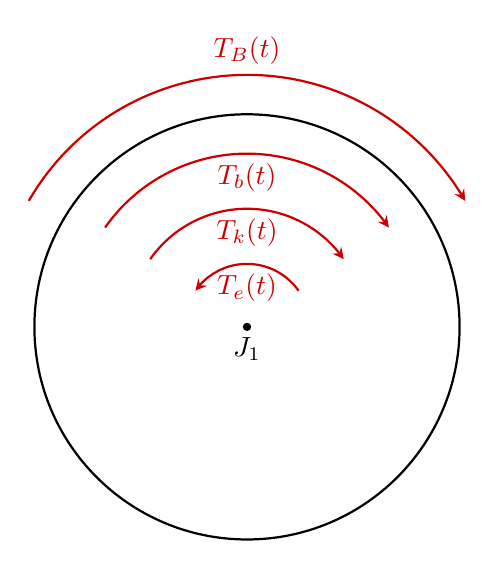
\begin{tikzpicture}[>=stealth, thick]
      \draw (0,0) circle (2.7);
      \fill (0,0) circle (1.5pt) node[below] {$J_1$};
      % T_b: clockwise about the centre
      \draw[->, red!80!black] (145:2.2) arc (145:35:2.2) node[midway, below] {$T_b(t)$};
      % T_k: clockwise about the centre
      \draw[->, red!80!black] (145:1.5) arc (145:35:1.5) node[midway, below] {$T_k(t)$};
      % T_e: counterclockwise about the centre
      \draw[->, red!80!black] (35:0.8) arc (35:145:0.8) node[midway, below] {$T_e(t)$};
      % T_B: clockwise around the outside
      \draw[->, red!80!black] (150:3.2) arc (150:30:3.2) node[midway, above] {$T_B(t)$};
    \end{tikzpicture}
    \caption{Free Body Diagram of Rotor}
  \end{minipage}\hfill
  \begin{minipage}[b]{0.48\linewidth}
    \centering
    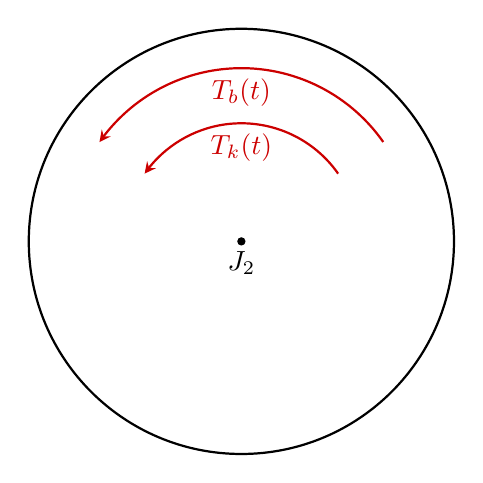
\begin{tikzpicture}[>=stealth, thick]
      \draw (0,0) circle (2.7);
      \fill (0,0) circle (1.5pt) node[below] {$J_2$};
      % T_b, T_k: counterclockwise about the centre
      \draw[->, red!80!black] (35:2.2) arc (35:145:2.2) node[midway, below] {$T_b(t)$};
      \draw[->, red!80!black] (35:1.5) arc (35:145:1.5) node[midway, below] {$T_k(t)$};
    \end{tikzpicture}
    \caption{Free Body Diagram of Load}
  \end{minipage}
\end{figure}
\answer{}

\end{document}
